\newpage
\section{Motivation}
\label {sec:motiv}
In this section, we explain the developement process of a highly
available application in \tool. We discuss a possible  anomily under
eventual consistency and then explain the difficulties associated 
with the manual approaches for prevention techniques.
Lastly we will explain how by automating the process, \tool can liberate
the developers from all those problems.
Our ideas mentioned here, are completed in  section
\ref{sec:ctrt_language}, where we extend the tool with a language, to
specify \emph{any} kind of anomalies. 


%
%--- What is the application, what are the requirements 
%
\subsection{RDTs in Eventually Consistent Stores }
\begin{figure}[t]
        \centering
	\begin{subfigure}[b]{0.489\textwidth}
	\begin{lstlisting}
type Effect = String 
type State =  String 

read :: State -> (String,Maybe Effect)
read s = (s,Nothing)

write :: String -> ((),Maybe Effect)
write comment = ((),comment)

apply :: State -> Effect -> State 
apply s eff = in s ++ " - " ++ comment
	\end{lstlisting}
	\caption{A simple implementation}
	\label{subfig:comment_code}
	\end{subfigure}
	\hfill
	\begin{subfigure}[b]{0.475\textwidth}
	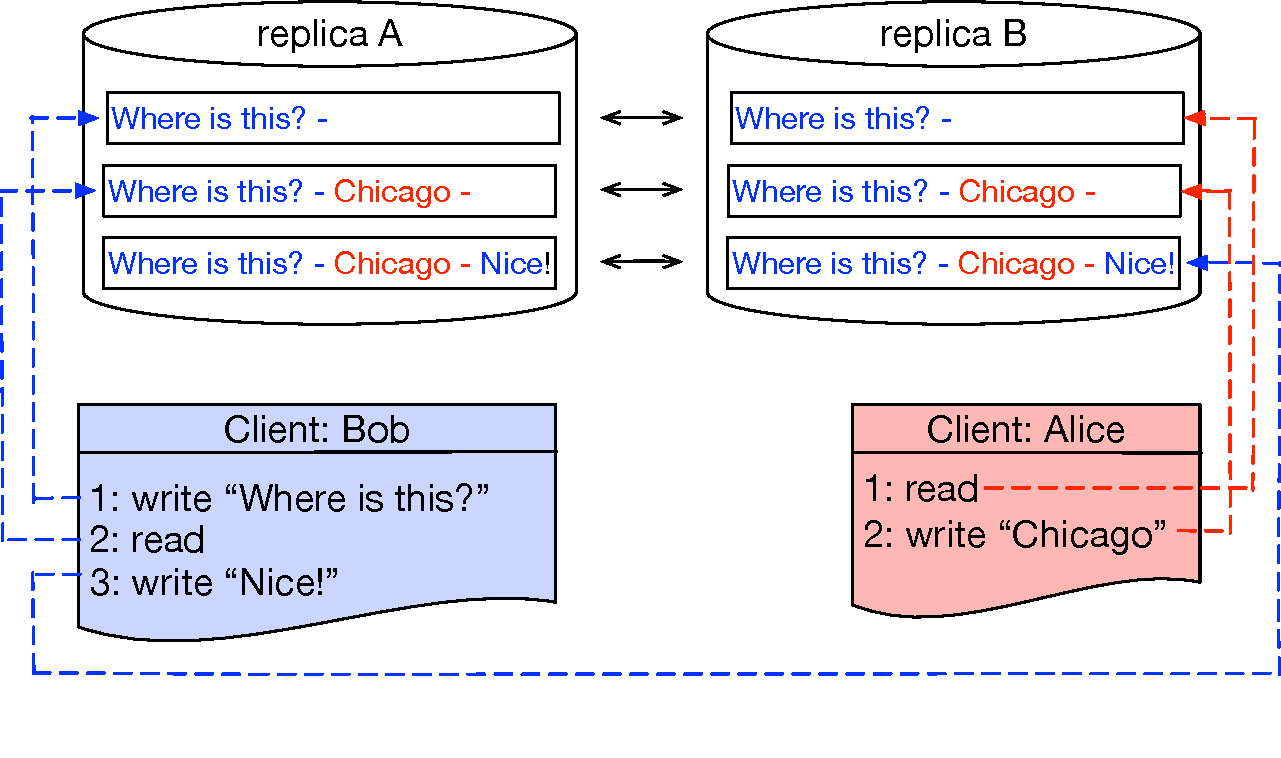
\includegraphics[scale=0.282]{Figures/comment_application.pdf}
	\caption{Example execution}
	\label{subfig:comment_example}
	\end{subfigure} 
\\ \hrulefill
\caption{A distributed application for comment section
management}
\label{fig:comment_app}
\end{figure}



Let's now consider a highly available comment
section management application, as part a photo sharing web site.
Figure \ref{subfig:comment_code} presnets implementation of such an application
in our system model. As explained in section \ref{sec:sys_model}, the
code is consisted of types \effectC{} and \stateC{}. Both types here are
defined as a strings, the former representing the text of a comment, and
the latter all the visible comments concatinated together.
Everytime a user calls the \writeC{} function to add a comment, an
\effectC{}
is generated and a \readC{} call simply
returns the \stateC{} of the object.

The \applyC{} function is given an effect, and is defined by the
developers to \emph{update} the objects' state.
Here the \applyC{} function simply pastes the 
included comment inside of  an effect, to the end of the current \stateC{}. As we mentioned earlier, we
completely separate the convergence semantics of the application  from the consistency
requirements. Since our focus is consistency here, we omit any conflict
resolution strategy in the code, however, developers (using roll-backs,
etc) can design the \applyC{} function to resolve conflicting
concurrent updates as they desire. 

Figure \ref{subfig:comment_example}, presents an example of how users
interact with the application. The example shows two clients, Bob and
Alice, that invoke operations on a comment section object. In the
setting Bob first writes a comment, which is routed to the replica A,
whose effect is then propagated and delivered to the replica B, where Alice's
first read operation is routed to next. Alice and Bob then keep talking
through more read and write events, whose order are marked in the
figure. 

Now let's assume Bob's read opration, instead of replica A, was routed
to another replica C, where the update from his first operation was not
present. This is \emph{lost-updates} anomaly, a very well-known
undesired behavior that is admitted in eventually consistent stores. 
Now developers are faced with the problem of preventing such an undesired
behavior, a task that as we will explain shortly, is difficult,
erorneous and heavily tangled with the application logic.
%
%--- What are the challenges implementing those reuquirements manually
%
\subsection{Ad-hoc Anomaly Prevention}
In this part, by referring to the modified code  presented in figure
\ref{fig:modified_code}, we will
explain a well-understood approach toward eliminating the lost\_update anomaly in
our comment manager application running on an EC store.

%tagging effects
First modification required in this technique is tagging effects with
unique identifiers, consisting of their originating sessions' id, and their
sequence number in them. This is used by replicas to
record the set of effects, that are alerady present locally
($line:1,2,5$). By this simple adjustment, the undesired anomaly would
be completely avoided, if operations would never be routed to replicas,
that do not contain all the effects from prior operations on that
session (let's call these effects the dependencies of
the operation). 

%blocking
Since operations do not have any control on which replica they are
routed to, the above property can be achieved, if operations that are
routed to a replica that does not contain their dependencies, wait
before execution until such effects become available at that replica.
This technique that is called {\bf blocking}, guarantees that the state
witnessed by oerations, 
is updated by a set of effects that is a \emph{superset} of the desired
dependencies.

Moreover, another technique called {\bf filteration} is used to further realize
the above idea. It basically separates the set off effects that have
arrived to the replica (available effects), and the effects who have
arrived and also been applied to the state (filtered effects).
By this separation, replicas can only apply effects to their state, if all
effects in session order with them, have already been applied to the
state. 
This way, replicas can record only the highest sequence
numbers from each session that they have applied to the state (since it
is guaranteed that the smaller ones are also applied)($line:3,6$). 
Figure \ref{fig:modified_code}, represents the blocking technique in the modified \readC{}
operation, where the result is only returned if the required
dependencies have already been applied to the state. Furthermore, the
filteration technique is used bu tge modified \applyC{} funciton, only
updates the state, if the sequence number of the given effect is
larger than the highest previously applied effect to the state precisly
by 1.
\begin{figure}[t]
	\centering
	\begin{subfigure}[t]{0.5\textwidth}
	\begin{lstlisting}
data Sess = Bob | Alice
type ID = (Sess,Int) 
type Effect= (ID,String)
type State = (String,Int,Int)
	
read :: ID -> State -> String
read (sess,seq) (st,sq1,sq2) = 
	case sess (*@\textcolor{blue}{of}@*) 
		Bob ->   if (seq==sq1+1) (*@\textcolor{blue}{then}@*) st
		         else read (sess,seq)(st,sq1,sq2)
		Alice -> if (seq==sq2+1) (*@\textcolor{blue}{then}@*) st
		         else read (sess,seq)(st,sq1,sq2)
	\end{lstlisting}		  
	\end{subfigure}
	%
	\hfill
        %
	\begin{subfigure}[t]{0.42\textwidth}
	\begin{lstlisting}[firstnumber=13]
	apply :: State -> Effect -> State 
	apply (st,sq1,sq2) ((sess,seq),cm) = 
	  case sess (*@\textcolor{blue}{of}@*) 
	    Bob ->   if (sq1==seq-1)
	             (*@\textcolor{blue}{then}@*) (st++cm,sq1+1,sq2)
	             else (st,sq1,sq2)
	    Alice -> if (sq2==seq-1)
	             (*@\textcolor{blue}{then}@*) (st++cm,sq1,sq2+1)
	             else (st,sq1,sq2)
	\end{lstlisting}		  
        \end{subfigure}

	\hrulefill
	\caption{Guarded Application to Prevent Lost-updates Anomaly
	When Serving Bob and Alice}
	\label{fig:modified_code}
\end{figure}




The above approach although is shown to work correctly, but as our
example showed, requires fundamentall changes in the code where 90\% of
the application was rewritten. Additionally, the modifications are
heavily tangled with the application logic which is problem for
developement of and reasoning about large
productions.

However, the major drawback of this approach is the fact that requires
constant alterations in the state of the application when the sessions
come and go. The application is now required to make
sure that a new field is created locally \emph{and} globally when 
new sessions are connected. This can extremely degrade the performance
of the system since it requires direct synchronization between replicas.
We have shown in detail how this adversely effects the performance in section
\ref{sec:eval}, where  we explain our experience in implementing
such an ad-hoc approach.

To make the matter worse, in addition to the above difficulties,
new anomalies are constantly found in the system, which requires
developers to come-up with non-trivial solutions. For example, in the
above application, another type of anomaly can occur when a third user
Chris, uses the application and submits a read, which is routed to a
replica D, that only contains the last write from Bob. Then Chris sees a
window containing "Me too!", which is an undesirable behavior. Now
developers are left with two options. First, they can try implementing
another non-trivial ad-hoc solution, which would further pollute the
application logic, making all the existing reasonings obsolete. Second,
they move the application completely to another store, that offers
stronger forms of consistency, such as causal consistency which would
prevent such anomalies. However, as we will show in section
\ref{sec:eval}, this would result in performance loss and potential
costumer loss.

%
%--- What is our alternative approach
%
\subsection{An Alternative}
We are now offering the developers with an alternative to the above
solutions. 
\tool, is a generic consistency managaement tool, running on
top of an off-the-shelf eventually consistent store, extending it to
a store with multiple configurable consistency levels. 
Developers can define a seperate environment for each operation at the
design stage, and configure each of them according to certain types of
anomalies, prevention of which is guaranteed by the tool. We have
relized this idea, following our observation that the prevention of basically all
types of anomalies, can be boiled down to two tasks,
filterataion and blocking. 


Our tool is equipped with a filteration mechanism, that periodically
refreshes the environments, and allows local effects at the replica to
enter each environment, if their presence would not cause the associated
anomaly occur. This way, \tool completely eliminates the
possibily of operations \emph{seeing effects that they are not supposed
to}, which is one important type of anomalies in distributed systems
(for example, in the above example Chris was not supposed to see Bob's
last comment since some effects were missing).


Similarly, the tool contains a blocker mechanism that makes sure all
operations are executed on their associated environment, only after the
environemnt contains the necessaity effects for preventing the associated
anomaly. Consequently, the operations will \emph{always see the effects
that they are supposed to}. This eliminates another type of anomalies in
the distributed systems, that the lost\_updates anomaly explained
previously, is an
example of. 


Using \tool, the developers are only required to configure environments
for each read operation, using a simple specification language that we
provide them with. The language is seeded with $\soZ$ $\visZ$ relations and allows
user to define different anomalous behaviors.  For example the
followings are the two consistency contracts written in our language,
regarding the two anomalies mentioned in this section 
\begin{smathpar}
\begin{array}{lllll}

1: & \forall (\eff,\eff'). & \eff \xrightarrow{\soZ} \eff' & \Rightarrow
& \eff
\xrightarrow {\visZ} \eff'  \\
2: & \forall(\eff,\eff'). & \eff \xrightarrow{\visZ;\visZ} \eff' &
\Rightarrow & \eff \xrightarrow {\visZ} \eff' 
\end{array}
\end{smathpar}


The first contract, that eliminates the possibility of lost\_updates,
tells the \tool to make sure that all effects that are in session order
to be also in vibility relation. This can be achieved by blocking
operations as explained above. 
The second contract, which prevents the second anomaly mentioned,
requires the system to make sure that if an effect is being made visible
to an operation, the operation should also witness all effects that were
visible to that effect.
In the next section, we will formally introduce our specification
language, and explain how two types of anomalies mentioned above, can be
specified in this language with different syntaxes.
\begin{wrapfigure}{i}{0.2\textwidth}
\centering
	\vspace{-10mm}
	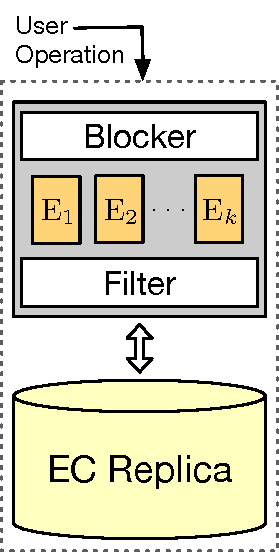
\includegraphics[scale=0.42]{Figures/outline.pdf}
	\label{fig:syncope_outline}
	\caption{\footnotesize \tool}
\label{fig:syncope_outline}
\vspace{-5mm}
\end{wrapfigure}
























